\section{Der Speicher}
\index{Speichermodell}
\label{sec:Speicher}

\subsection{Adressierungsarten}
\label{subsec:Adressierungsarten}
\index{Adressierungsarten}

Als RISC-orientierte Maschine, greift die UMach lediglich in zwei Situationen
auf den Speicher zu: zum Schreiben von Registerinhalten in den Speicher
(Schreibzugriff) und zum Lesen von Speicherinhalten in einen Register
(Lesezugriff).  Die \gls{Adressierungsart} beschreibt dabei, wie der Zugriff
auf den Speicher erfolgen sollte, bzw. wie die angesprochene Speicheradresse
angegeben wird. Anders ausgedrückt, beantwortet die Adressierungsart die Frage
\glqq wie kann eine Instruktion der Maschine eine Adresse angeben?\grqq. 

Die UMach Maschine kennt eine einzige Adressierungsart: die (register-)
indirekte Adressierung. Dabei werden alle Speicheradressen nicht direkt
angegeben, sondern es wird ein Register angegeben, der die Adresse beinhaltet.
Zum Beispiel, die Instruktion 
\begin{lstlisting}
 0x13 0x01 0x02 0x00
\end{lstlisting}
bedeutet nicht \glqq lade das Wort an der Adresse \texttt{0x02} in das Register
mit Nummer \texttt{0x01}\grqq, sondern \glqq lade das Wort, das an der Adresse
liegt, die in Register mit Nummer \texttt{0x02} angegeben ist, in das Register
mit Nummer \texttt{0x01}\grqq. Das entpricht der Instruktion
\begin{lstlisting}
 LW R1 R2
\end{lstlisting}
Analog gilt für Schreibbefehle.


\subsection{Speicherstruktur}
\index{Speicherstruktur}

Der Speicher der UMach Maschine hat zur Laufzeit eine bestimmte Struktur, bzw.
wird in bestimmten Bereichen unterteilt. Diese Bereiche sind
\begin{enumerate}
 \item Unterbrechungstabelle
 \item Programm und Daten
 \item Stack
\end{enumerate}

Siehe auch die Abbildung \ref{fig:Speicherstruktur} auf der Seite
\pageref{fig:Speicherstruktur}.

\begin{figure}[htp]
 \centering
 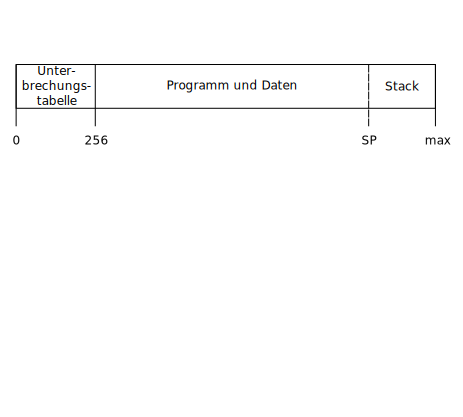
\includegraphics{./img/UMach-Speicherstruktur}
 \caption[Speicherstruktur]{Speicherstruktur zur Laufzeit}
 \label{fig:Speicherstruktur}
\end{figure}



\subsubsection{Unterbrechungstabelle}
\index{Unterbrechungstabelle}
\label{subsubsec:Unterbrechungstabelle}

Die Unterbrechungstabelle besteht aus einer Reihe von Sprungadressen zum
ausführbaren Code, bzw. zu sogenannten Unterbrechungsroutinen, oder \glqq
interrupt handlers\grqq, die in Ausnahmefällen ausgeführt werden sollen. Jedes
mal, wenn eine Ausnahmesituation auftritt (meistens eine Fehlersituation), wird
intern ein Unterbrechungssignal erzeugt, das mit einer Kennnummer
(Unterbrechungsnummer) versehen ist. Die Unterbrechungsnummer wird als Index in
dieser Tabelle verwendet.

Hier ist die Rede von Unterbrechungen, die direkt mit der Ausführung von
Instruktionen verbunden sind (Hardware Interrupts). Sie können entweder von der
Maschine selbst erzeugt werden, wie z.B. im Falle einer Division durch Null,
oder im Falle, dass eine unerlaubte Speicheradresse verwendet wird, oder sie
können unter Programmkontrolle erzeugt werden. Siehe auch den Abschnitt
\ref{sec:Unterbrechungen}, ab der Seite \pageref{sec:Unterbrechungen}.


Die Unterbrechungstabelle wird von der Maschine nicht gefüllt, sondern es ist
Sache der Software, die entsprechenden Stellen im Speicher zu füllen und
entsprechende Funktionalität zur Verfügung zu stellen. Wird eine solche Adresse
nicht gesetzt, d.h. ist der entsprechende Tabelleneintrag auf Null gesetzt, so
reagiert die Maschine auf die Ausnahmesituation mit seiner Standardfunktion: die
Maschine hält an. Für weitere Informationen bzgl. der Fehlerbehandlung siehe den
Abschnitt \ref{sec:Unterbrechungen}, ab der Seite \pageref{sec:Unterbrechungen}.


Die Unterbrechungstabelle enthält 64 Einträge, wobei nicht alle Einträge belegt
sein müssen. Jeder Eintrag beträgt 32 Bit (gleich lang wie ein Register). Jeder
Index in der Tabelle entspricht einer Unterbrechungsnummer (Hardware Interrupt).
Die Einträge werden für bestimmte Ausnahmefälle verwendet, die in der Tabelle
\ref{tab:Unterbrechungstabelle} angegeben sind.


\begin{longtable}{>{\ttfamily}ll}
\caption{Unterbrechungsnummer}
\label{tab:Unterbrechungstabelle}
\\\toprule
 0 & Division durch Null \\
 1 & Überlauf \\
 99 & Noch nicht fertig
\\\bottomrule
\end{longtable}



\subsubsection{Der Stack}
\label{subsubsec:Stack}
\index{Stack}

Der Stack ist ein spezieller Bereich im Speicher. Dieser Bereich fängt am Ende
des Speichers mit der größten Adresse an und erstreckt sich bis zur derjenigen
Adresse, die im Register \texttt{SP} gespeichert ist. Die Stack-Größe ist damit
dynamisch, denn das Register \texttt{SP} wird sowohl durch die Instruktionen
\opref{PUSH} und \opref{POP}, als auch direkt vom Programmierer geändert.

Das Wachsen\index{Stack!Wachsen} des Stacks bedeutet, dass das Register
\texttt{SP} immer kleinere Werte annimmt. Das Schrumpfen\index{Stack!Schrumpfen}
des Stacks bedeutet, dass \texttt{SP} immer größere Werte annimmt. Wird
versucht, den Inhalt von \texttt{SP} kleiner Null oder größer als die maximale
Speicheradresse zu setzen, so wird dies von der Maschine verweigert und als
Fehler im Register \texttt{ERR} signalisiert.

Beim Hochfahren der Maschine, wird das Register \texttt{SP} auf die
maximal-erreichbare Speicheradresse plus Eins gesetzt. Damit können keine Werte
gelesen werden, bevor Werte geschrieben wurden.

